
\documentclass[letterpaper,11pt]{article}
\usepackage[utf8]{inputenc}
\usepackage[spanish]{babel}
\usepackage{mathtools}
\usepackage{graphicx}
\usepackage{hyperref}
\usepackage{tikz}
\usepackage{amsmath}
\usepackage{latexsym}
\usepackage{amssymb}
\usepackage{algorithm}
\usepackage[noend]{algpseudocode}

\begin{document}

\title{Estructura de datos\\\Large Algoritmos de búsqueda en gráfos\\\small Actividad 10}
\author{Dagoberto Quevedo}
\maketitle

\begin{abstract}
En esta actividad se describen métricas y algoritmos de búsqueda y recorrido en grafos. Se procede a realizar la implementación en Python que genera un grafo aleatorio y procede a calcularse su diámetro, densidad, distancia con el algoritmo de Dijkstra y centralidad de grado, adicional se implementa un método de búsqueda en profundidad.
\end{abstract}

\section{Representación eficiente de grafos}

Un grafo con $n$ vértices puede se almacenada en un matriz de adyacencias, pero sólo resulta eficiente si la densidad del grafo es alta, dado que almacenar un grafo en una matriz ocupa $n^2$ de espacio, si $m\ll n^2$ la mayoría de los espacios reservados son cero. La forma de optimizar el espacio de almacenamiento es usar listas de adyacencia, dado un arreglo $a[]$, cada elemento contiene un lista dinámica $a[i]$ con los vértices adyacentes a $i$; el tamaño de esta estructura es $\mathcal{O}(n+m)\leq \mathcal{O}(m) = \mathcal{O}(n^2)$ \cite{Schaeffer2020}. 

\section{Métricas y algoritmos en gráfos}

La \textit{densidad} es el número máximo de posible de aristas es,

\begin{equation}
m_{\max} = \binom{n}{2} = \frac{n(n-1)}{2}, 
\end{equation}

entonces la densidad $\delta(G)$, es,
\begin{equation}
\delta(G) = \frac{m}{m_{\max}} = \frac{m}{\binom{n}{2}},
\label{eq:densidad}
\end{equation}

por lo que un grafo es denso si $\delta(G)\approx 1$, y un grafo poco denso si $\delta(G) \ll 1$. El \textit{grado}  de un vértice $i$,

\begin{equation}
\eta(i) = |\{ j \in V : (i,j) \in E \}|
\label{eq:grado}
\end{equation}

La distancia $\ell(a,b)$ entre $a$ y $b$ es el largo mínimo de todos los caminos de $a$ a $b$ el \textit{diametro} $\gamma(G)$ de un grafo $G$, el la distancia máxima en todo el grafo,

\begin{equation}
\gamma(G) = \max_{a,b\in V}\ell(a,b).
\label{eq:distancia}
\end{equation}

La \textit{centralidad de grado} es dada por,

\begin{equation}
	i_{\max} = \max_{i\in V} \eta(i).
	\label{eq:centralidad}
\end{equation}

%n = len(self.V)
  %      m = sum(self.E.values()) / 2.0
    %    dens = m / ((n * (n - 1))/ 2.0)


\subsection{Búsqueda en profundidad}

La búsqueda en profundidad (DFS por sus siglas en inglés \textit{Depth-First Search}), explora los posibles vértices (desde un vértice inicial) hacia abajo de cada rama antes de retroceder. Esta propiedad permite que el algoritmo se implemente recursivamente \cite{Papadimitriou1993}. En general el método realiza las siguientes operaciones: 1) Marcar el vértice actual como visitado; 2) Explorar cada vértice adyacente al nodo actual que no haya sido visitado aún. El algoritmo recursivo se definiria como sigue,

\begin{algorithm}
\caption{Búsqueda en profundidad}\label{euclid}
\begin{algorithmic}[1]
\Procedure{DFS($v$,$L$)}{}
\State $L= L\cup \{v\}$

 \For {$w \in \{j \in V : (i,j) \in E \}$}
\State DFS($w$,$L$)
\EndFor
\Return $L$
\EndProcedure
\end{algorithmic}
\end{algorithm}


\section{Implementación computacional}

Se realiza una implementación computacional dado un valor $m$ que determina el numero de elementos en $V$, generar un grafo no dirigido $G=(V,E)$, donde las aristas $(i,j)\in E, i,j\in V$ se asignan desde una probabilidad uniforme de conexión entre sus elementos definida por $p_{ij}$. Una vez generado calcular lo siguiente: a) diámetro, b) densidad, distancias, usando el algoritmo de Dijkstra y c) determinar el elemento más y menos central del grafo a partir de la centralidad de grado, donde el grado de un elemento $i$ es dado por $\deg(i) = \sum_{j\in V} A_{ij}$, siendo $A$ la matriz de adyacencias. Adicional se implementa una búsqueda en profundidad recursiva. Finalmente realizar la representación gráfica del grafo generado.

\subsection{Resultados}

\begin{figure}[h]
 \centering
  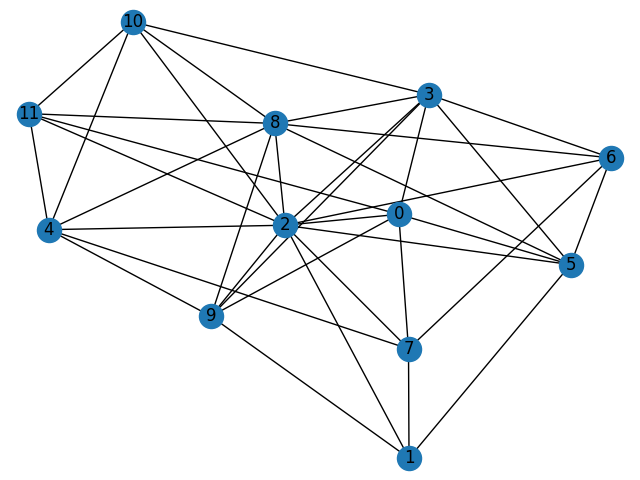
\includegraphics[width=10cm]{out.png}
  \caption{Resultado de la estructura de gráfo generada aleatoriamente}
  \label{fig:bs}
\end{figure}

\begin{thebibliography}{0} 
  \bibitem{Papadimitriou1993} Christos H. Papadimitriou, \textit{Computational Complexity}, Addison-Wesley Professional, 1993.
  \bibitem{Knuth1998} Donald Knuth, \textit{Sorting and searching}, The Art of Computer Programming, Addison-Wesley Professional, 1998.
  \bibitem{Schaeffer2020} Elisa Schaeffer, \textit{Modelos computacionales}, Complejidad computacional de problemas y el análisis y diseño de algoritmos, notas de curso, 2020.
\end{thebibliography}


\end{document}


